\documentclass[10pt, aspectratio=169]{beamer}

% Load the theme/package from the subfolder
\usepackage{Styles/beamerthemeUCSDContact}                    

% Packages 
\setbeamercovered{transparent}
\usepackage{hyperref}
\usepackage{datetime}

% Hyperlink Setup
\hypersetup{hidelinks}

% Title Slide
\title{Sampling-Based and Contact-Implicit Nonprehensile \\ Manipulation using Signed Distance Functions}
\pis{Nikola Raicevic}                 
\author{PI: Nikolay Atanasov}                    
\institute{Department of Electrical and Computer Engineering\\University of California San Diego}
\newdate{mydate}{04}{09}{2025}
\date{\displaydate{mydate}}

% % --- Auto outline at each section start ---
% \AtBeginSection[]{\begin{frame}{Outline}
%     \tableofcontents[
%       currentsection,
%       sectionstyle=show/shaded,
%       subsectionstyle=show/show/shaded
%     ]
%   \end{frame}}

\begin{document}

% --- Title slide ---
\begin{frame}[plain]\titlepage\end{frame}

% % --- Full outline ---
% \begin{frame}{Outline}
%   \tableofcontents % or [hideallsubsections]
% \end{frame}

% --- Motivation & Background ---
\section{Motivation \& Background}
% Motivation
\begin{frame}{Motivation}
  \begin{columns}[T,onlytextwidth]
    \begin{column}{0.5\textwidth}
      \small
      \textbf{Real-world help requires touch}
      \begin{itemize}\setlength{\itemsep}{0.35em}
        \item Homes are cluttered and unpredictable, intentional contact makes behavior robust
        \item Safe assistance around people and fragile items needs gentle, controlled touch
      \end{itemize}

      \vspace{0.5em}
      \textbf{Everyday tasks that depend on contact}
      \begin{itemize}\setlength{\itemsep}{0.35em}
        \item \emph{Cleaning \& organizing}
        \item \emph{Making a smoothie}
        \item \emph{Assisting the elderly}
        \item \emph{Quick household fixes}
        \item \emph{Kitchen help}
      \end{itemize}
    \end{column}

    \begin{column}{0.3\textwidth}
    \end{column}
  \end{columns}
\end{frame}

% Background
\begin{frame}{Background}
\begin{columns}
  \begin{column}{0.56\textwidth}
    \small
    \begin{itemize}
      \item \textbf{Contact changes the world state} \\
      Touch creates forces and \emph{mode switches} (no contact / pushing / pulling / lifting-off) $\rightarrow$ discontinuities
      \vspace{0.5em}
      \item \textbf{Classical planners fall short} \\ 
      They operate in continuous spaces and assume collision-free motion, treating objects as obstacles, not tools
      \vspace{0.5em}
      \item \textbf{What we need} \\ 
      Let the robot \emph{discover} useful contacts (when/where/how) as part of the plan—no brittle, pre-fixed contact scripts
    \end{itemize}
  \end{column}
  \begin{column}{0.44\textwidth}
    \centering
    {\bfseries Xarm6 with Tee}\\[0.3em]
    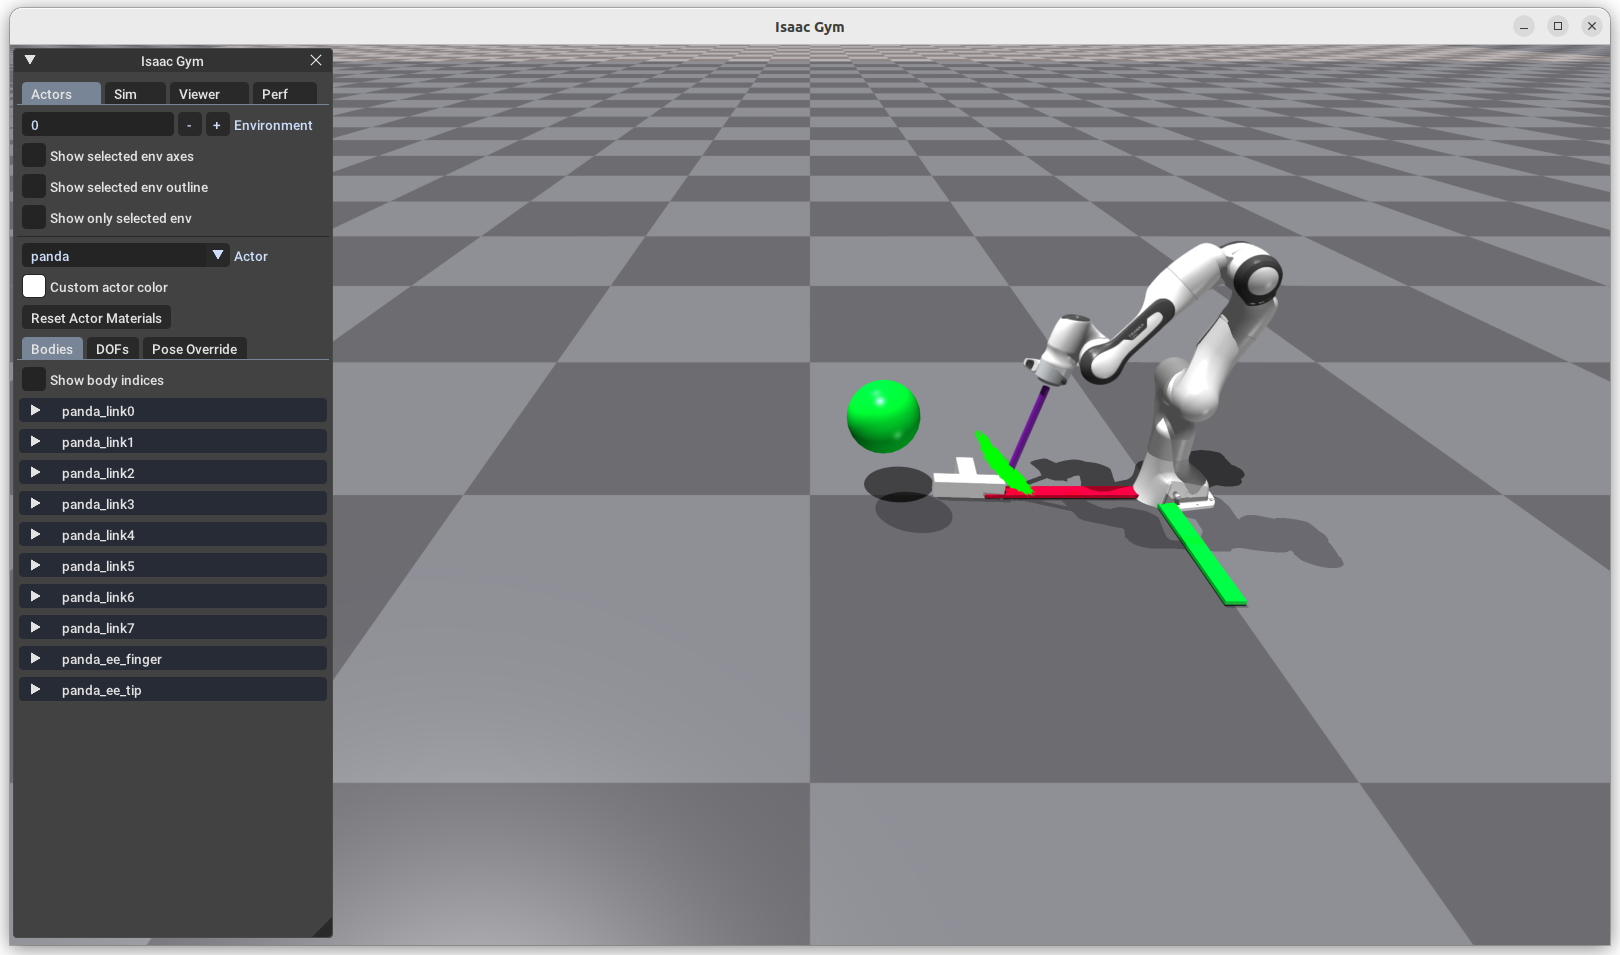
\includegraphics[width=\linewidth]{Figures/Xarm6_tee.png}\\
    \vspace{0.25em}
    \scriptsize Example: an arm uses touch to achieve a goal rather than avoiding it
  \end{column}
\end{columns}
\end{frame}

% Related Work
\begin{frame}{Related Work}
    \small
    \begin{columns}[T,onlytextwidth]
    \begin{column}{0.33\textwidth}
        % -------- Learning-based --------
      \textbf{Learning-based}
          \begin{itemize}
            \item \emph{Pros:} learns rich, non-linear policies; end-to-end; adapts with more data
            \item \emph{Cons:} data-demanding; reward shaping; sim-to-real/transfer gaps
            \item \emph{Limits:} tends to overfit object/task; generalization to new shapes is hard
            \item \emph{Example:} \href{https://proceedings.mlr.press/v270/he25c.html}{\footnotesize Visual Manipulation with Legs}\,\footnotemark[1]
          \end{itemize}
        \end{column}
        
        % -------- Sampling-based --------
        \begin{column}{0.33\textwidth}
          \textbf{Sampling-based}
          \begin{itemize}
            \item \emph{Pros:} handles multi-modal choices; real-time re-planning; no gradients needed
            \item \emph{Cons:} model-free variants \emph{sample blindly}; cost shaping heavily influences outcomes
            \item \emph{Limits:} no built-in guidance for \emph{where/when} to contact; many rollouts for delicate timing
            \item \emph{Example:} \href{https://arxiv.org/abs/2409.15610}{\footnotesize DIAL-MPC \,\footnotemark[2]}
          \end{itemize}
        \end{column}
        
        % -------- Model-based --------
        \begin{column}{0.33\textwidth}
          \textbf{Model-based}
          \begin{itemize}
            \item \emph{Pros:} interpretable; geometry/dynamics aware; efficient when models match reality
            \item \emph{Cons:} explicit contact/complementarity can be brittle
            \item \emph{Limits:} fine-tuning per object shape/scene; manual constraint engineering
            \item \emph{Example:} model-based pushing \href{https://arxiv.org/abs/2502.01055}{\footnotesize CRISP\,\footnotemark[3]}
          \end{itemize}
    \end{column}
    \end{columns}
    
  % References in footnotes
  \footnotetext[1]{\scriptsize He, X., et al. (2025).
  \emph{\href{https://proceedings.mlr.press/v270/he25c.html}{Visual Manipulation with Legs}}.
  Proceedings of The 8th Conference on Robot Learning, PMLR}
  \footnotetext[2]{\scriptsize Xue, H., et al.(2024).
  \emph{\href{https://arxiv.org/abs/2409.15610}{Full-Order Sampling-Based MPC for Torque-Level Locomotion Control via Diffusion-Style Annealing}}}
  \footnotetext[3]{\scriptsize Li, Y., et al. (2025).
  \emph{\href{https://arxiv.org/abs/2502.01055}{On the Surprising Robustness of Sequential Convex Optimization for Contact-Implicit MP}}}
\end{frame}

% Related Work: Our Approach
\begin{frame}{Related Work: Our Approach}
  \textbf{What Is Missing?}
  \begin{itemize}
    \item Geometry-aware guidance without per-object re-training or manual mode schedules
    \item A planner that \emph{discovers} contact strategy (where/when/how) based on the task
    \item Generalization across shapes/layouts with sample efficiency and interpretability
  \end{itemize}

  \vspace{0.8em}
  \textbf{Our Approach:}
  \begin{itemize}
    \item Contact-implicit, geometry-aware sampling model-predictive control using Signed Distance Function (SDF) for guidance
    \item Push from start $\rightarrow$ goal with \emph{no re-training} for new shapes, \emph{no blind sampling}, minimal manual constraints, and no task-specific data
  \end{itemize}
\end{frame}

% --- Problem Formulation ---
\section{Problem Formulation}
\begin{frame}{Problem Formulation}
  \begin{columns}[T]
    \begin{column}{0.6\textwidth}
        \textbf{Objective:} Given a robot's initial configuration $q_0$ and target object's signed distance function $\phi(p)$, find a sequence of controls $u_{0}$ to relocate an object from start pose $T_0$ to goal pose $T^*$
        \medskip

        \textbf{Given:}
        \begin{itemize}
            \item $T_0$ — Initial object pose
            \item $T^*$ — Goal object pose
            \item $q_0$ — Initial robot configuration
            \item $u_{0}$ — Initial robot controls (i.e. velocities,torques)
            \item $\phi(p)$ — Signed distance function (SDF) of the target object  
        \end{itemize}
    \end{column}

    \begin{column}{0.4\textwidth}
      \centering
      {\bfseries Problem Setup}\\[0.5em]
      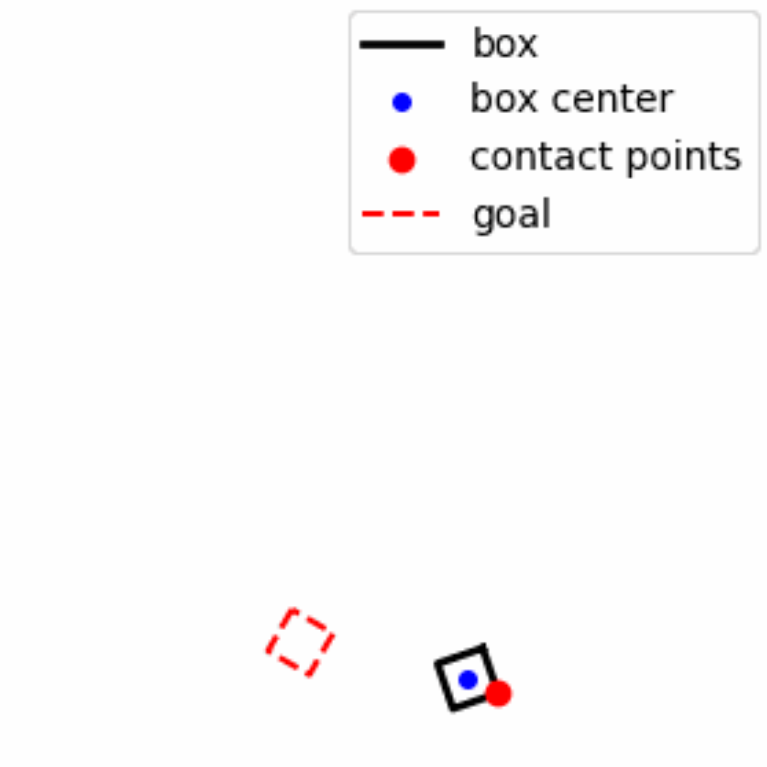
\includegraphics[width=\textwidth]{Figures/problem_formulation.png}
    \end{column}
  \end{columns}
\end{frame}

% --- SDF Function ---
\begin{frame}{Signed Distance Function}
  \begin{columns}[T,onlytextwidth]
    % ---------------- LEFT: text ----------------
    \begin{column}{0.35\textwidth}
      \vspace{8.0em}
      \textbf{SDF sign convention} \\
      $\phi(\mathbf{p}) > 0$ outside the object,\; \\
      $\phi(\mathbf{p}) = 0$ on the surface,\; \\
      $\phi(\mathbf{p}) < 0$ inside.
    \end{column}

    % ---------------- RIGHT: figures ----------------
    \begin{column}{0.65\textwidth}
      \centering

      % ---------- top row ----------
      \begin{minipage}{\linewidth}
        \begin{minipage}{0.5\linewidth}
          \centering
          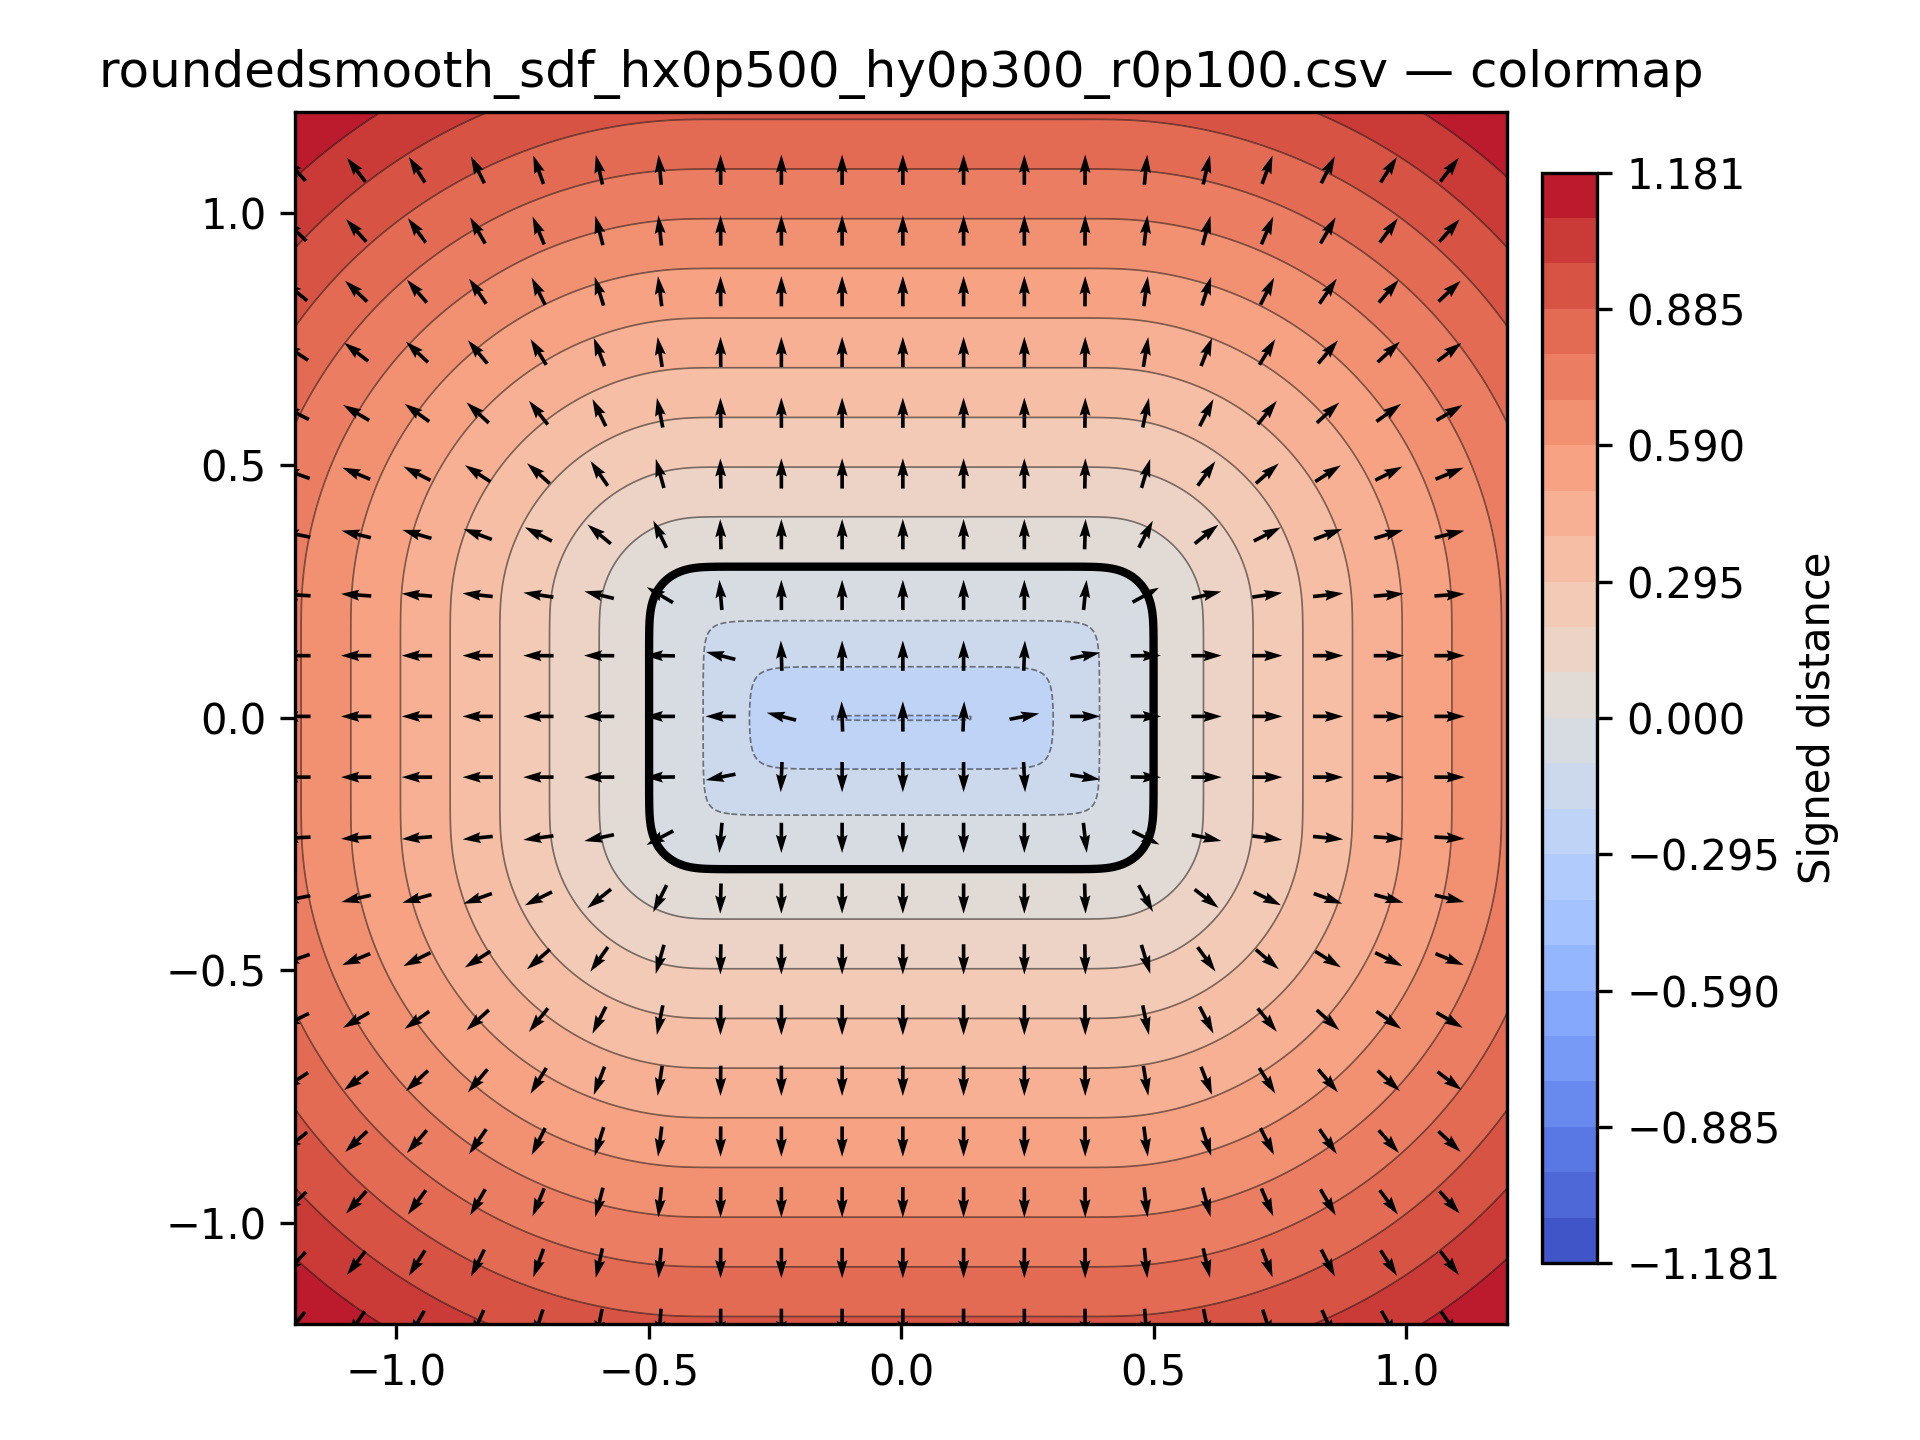
\includegraphics[width=\linewidth]{Figures/roundedsmooth_sdf_hx0p500_hy0p300_r0p100_cmap.png}\\[-0.2em]
          \scriptsize Rounded box — field
        \end{minipage}\hfill
        \begin{minipage}{0.5\linewidth}
          \centering
          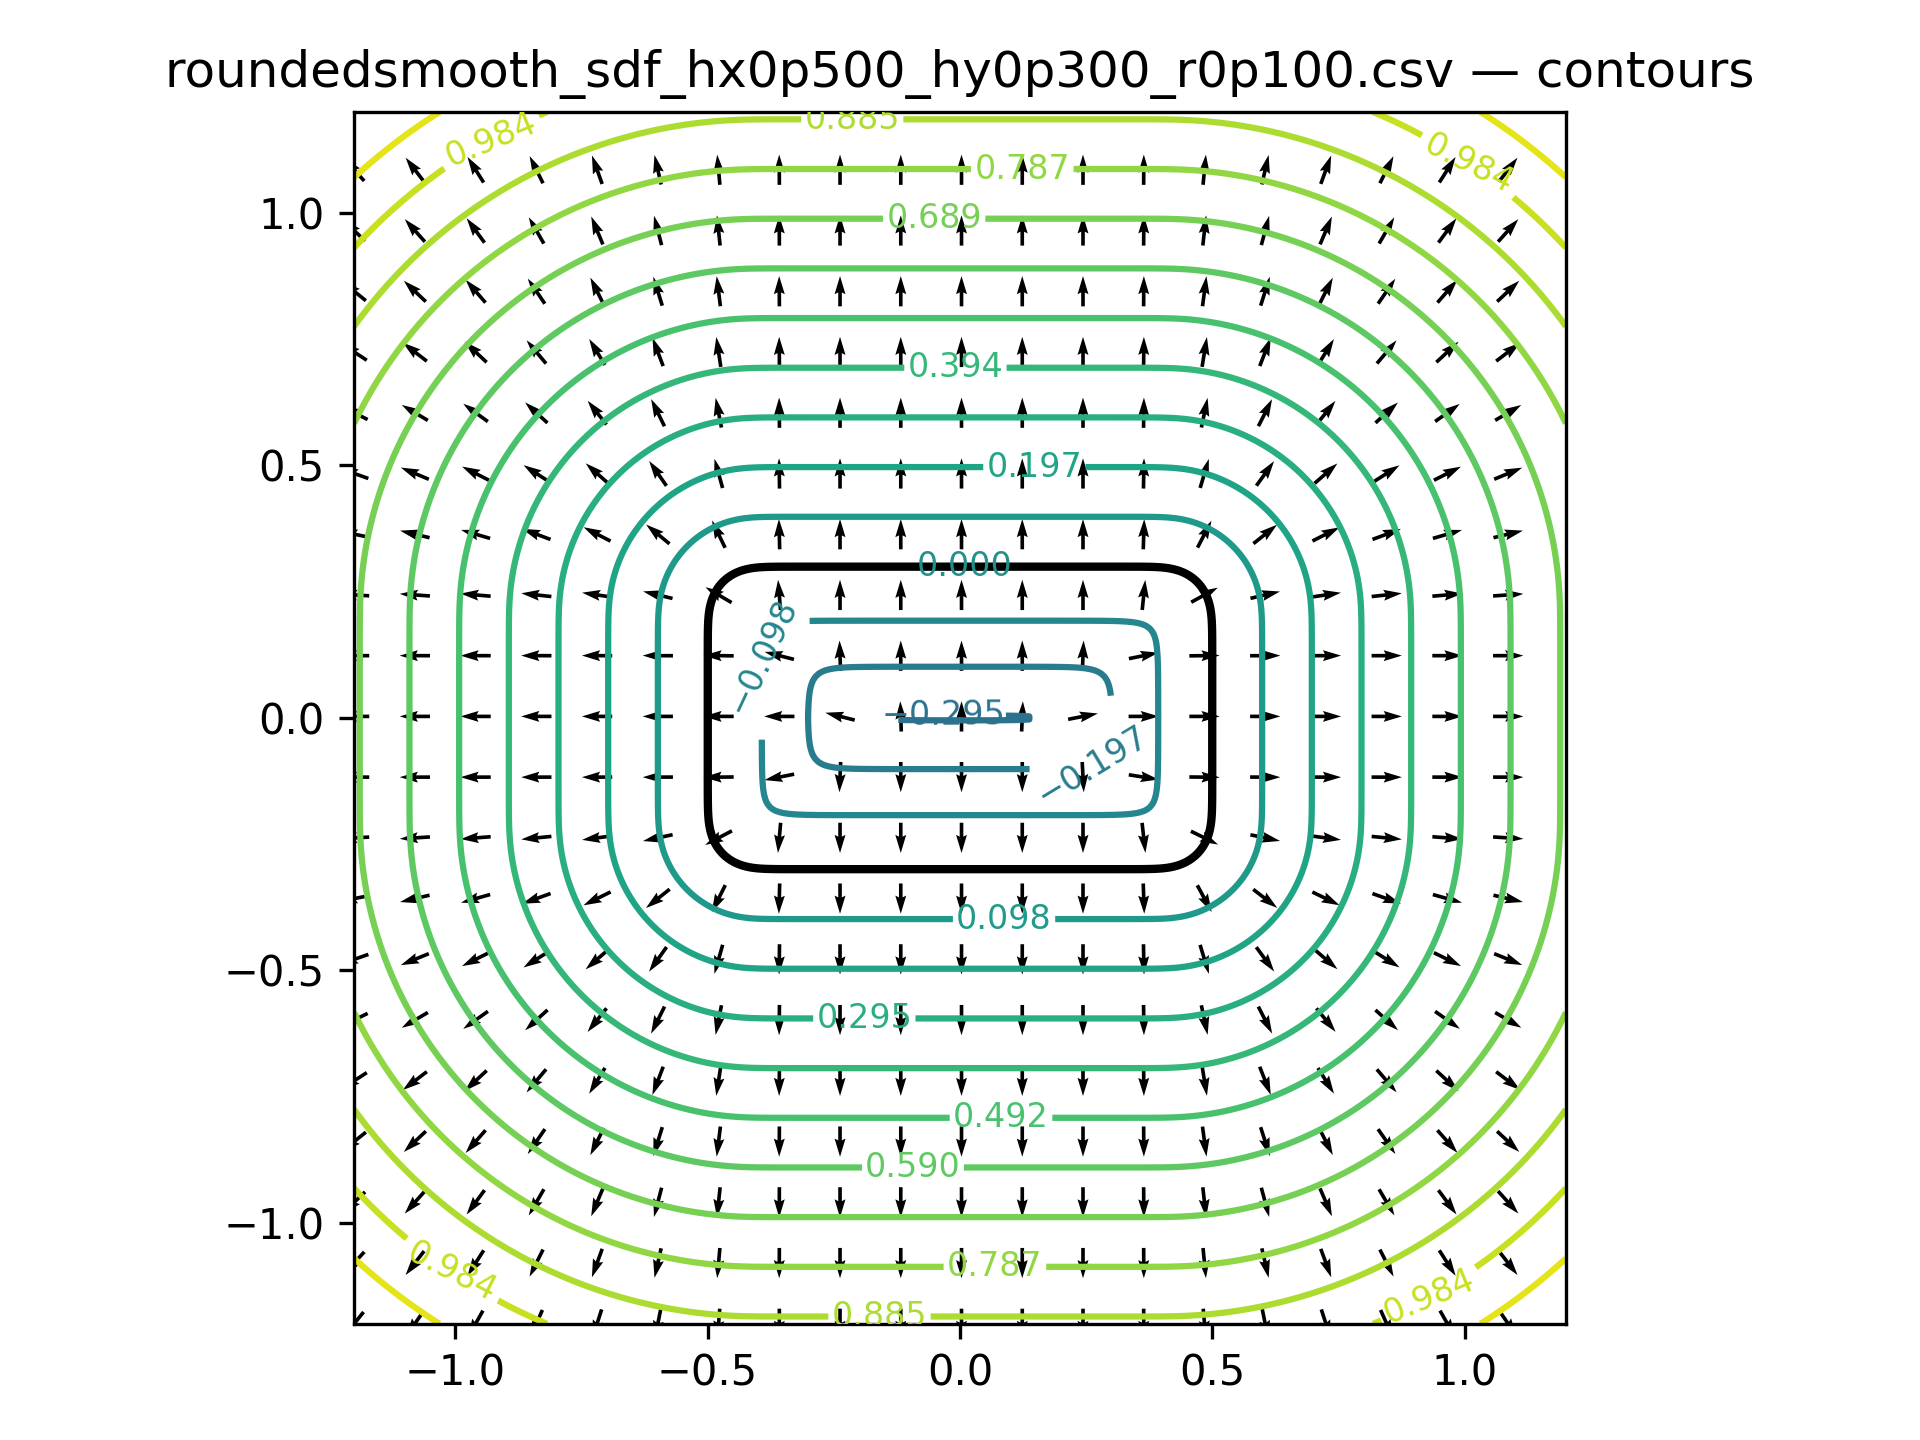
\includegraphics[width=\linewidth]{Figures/roundedsmooth_sdf_hx0p500_hy0p300_r0p100_contour.png}\\[-0.2em]
          \scriptsize Rounded box — contour
        \end{minipage}
      \end{minipage}
      \vspace{0.6em}

      % ---------- bottom row ----------
      \begin{minipage}{\linewidth}
        \begin{minipage}{0.5\linewidth}
          \centering
          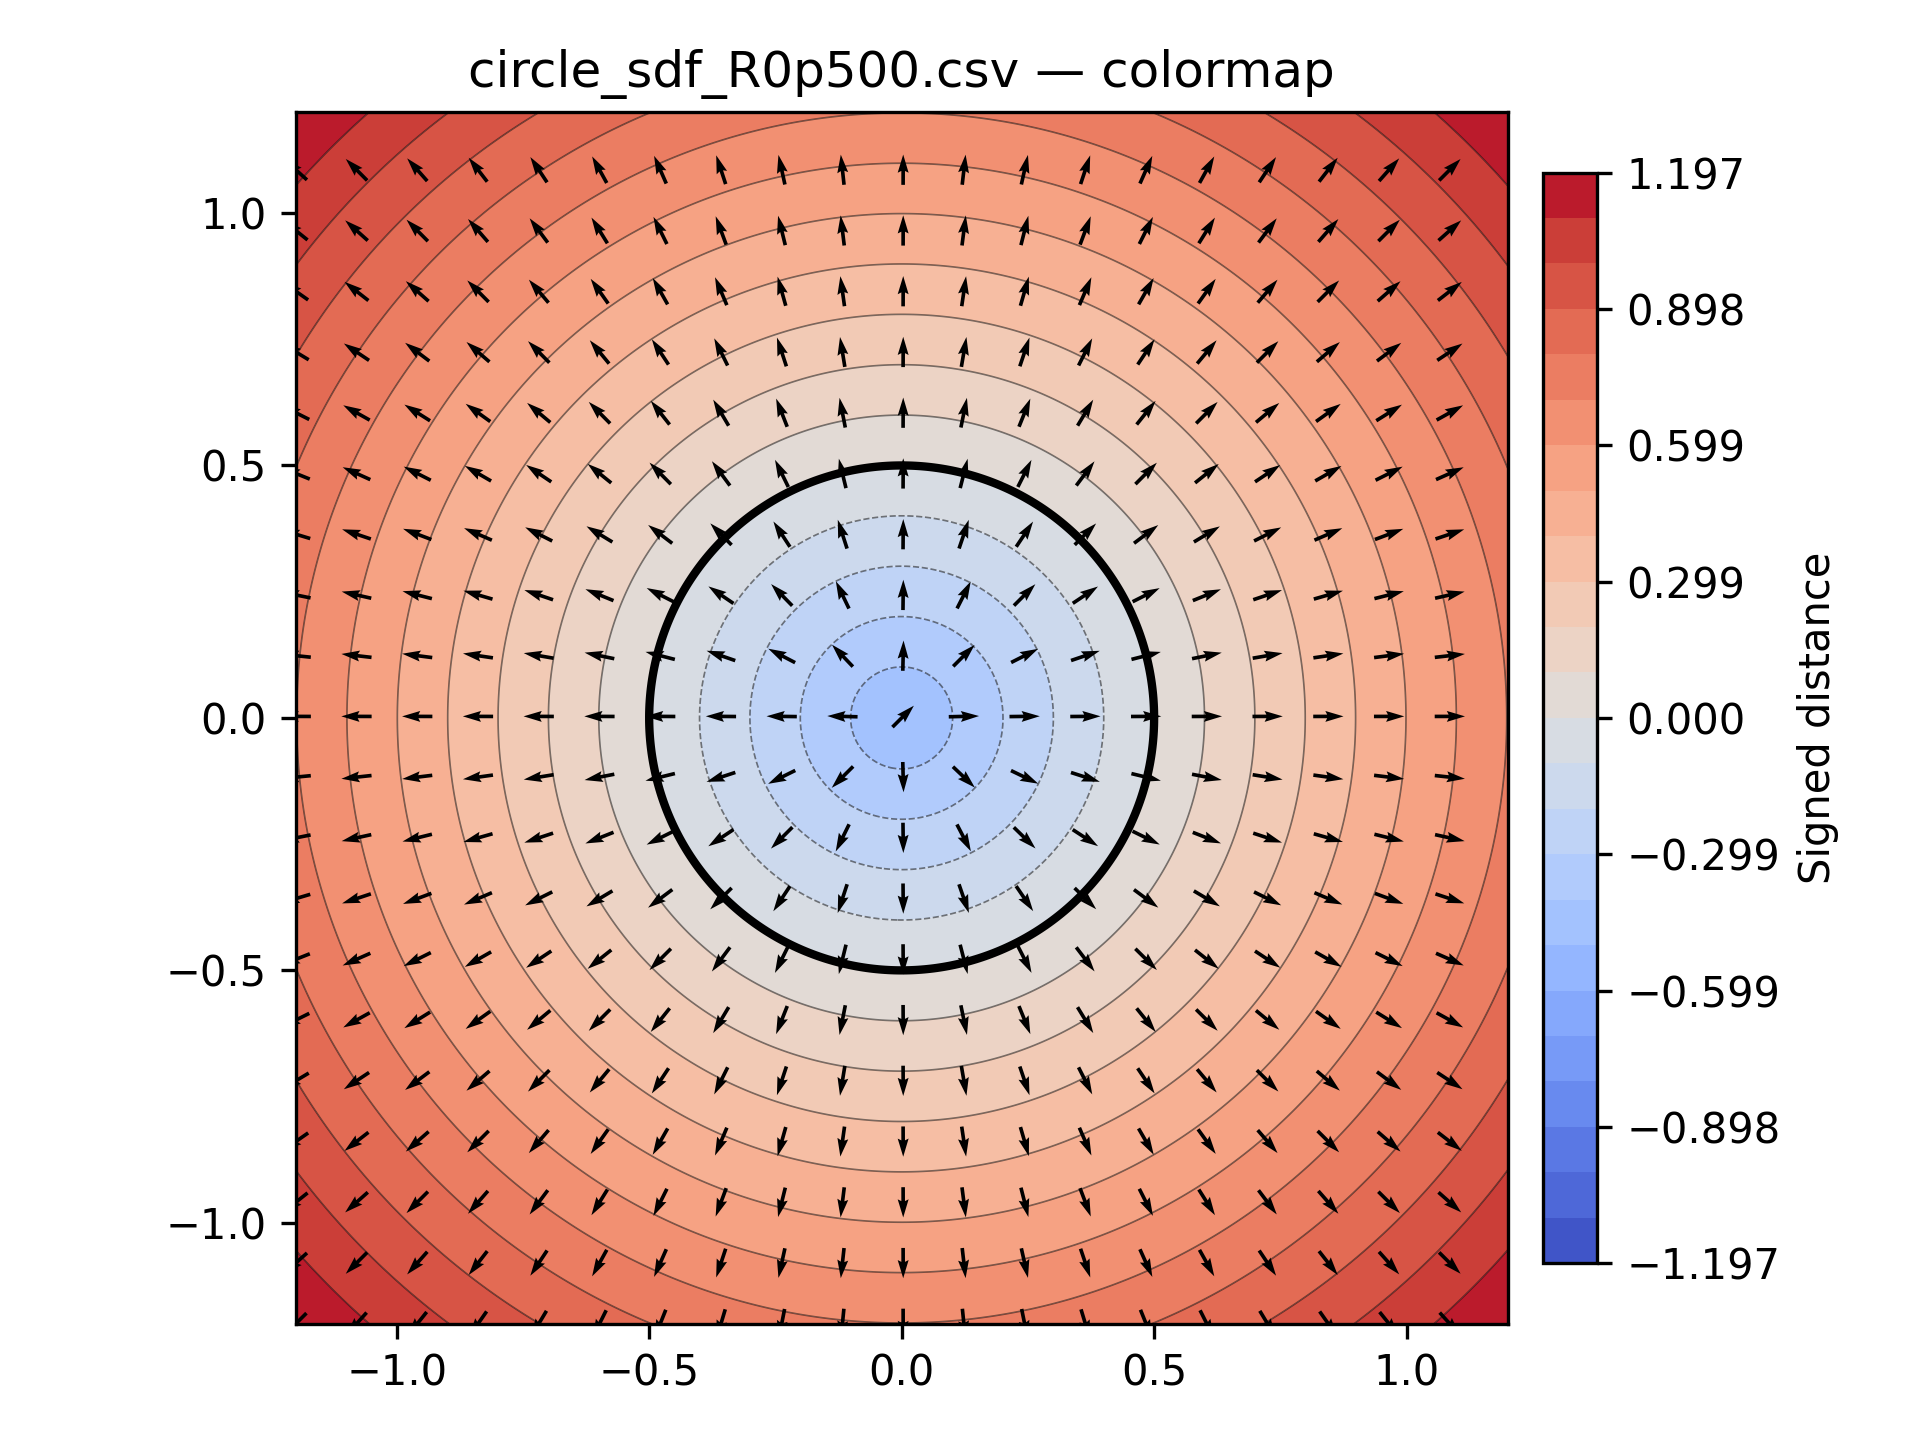
\includegraphics[width=\linewidth]{Figures/circle_sdf_R0p500_cmap.png}\\[-0.2em]
          \scriptsize Circle — field
        \end{minipage}\hfill
        \begin{minipage}{0.5\linewidth}
          \centering
          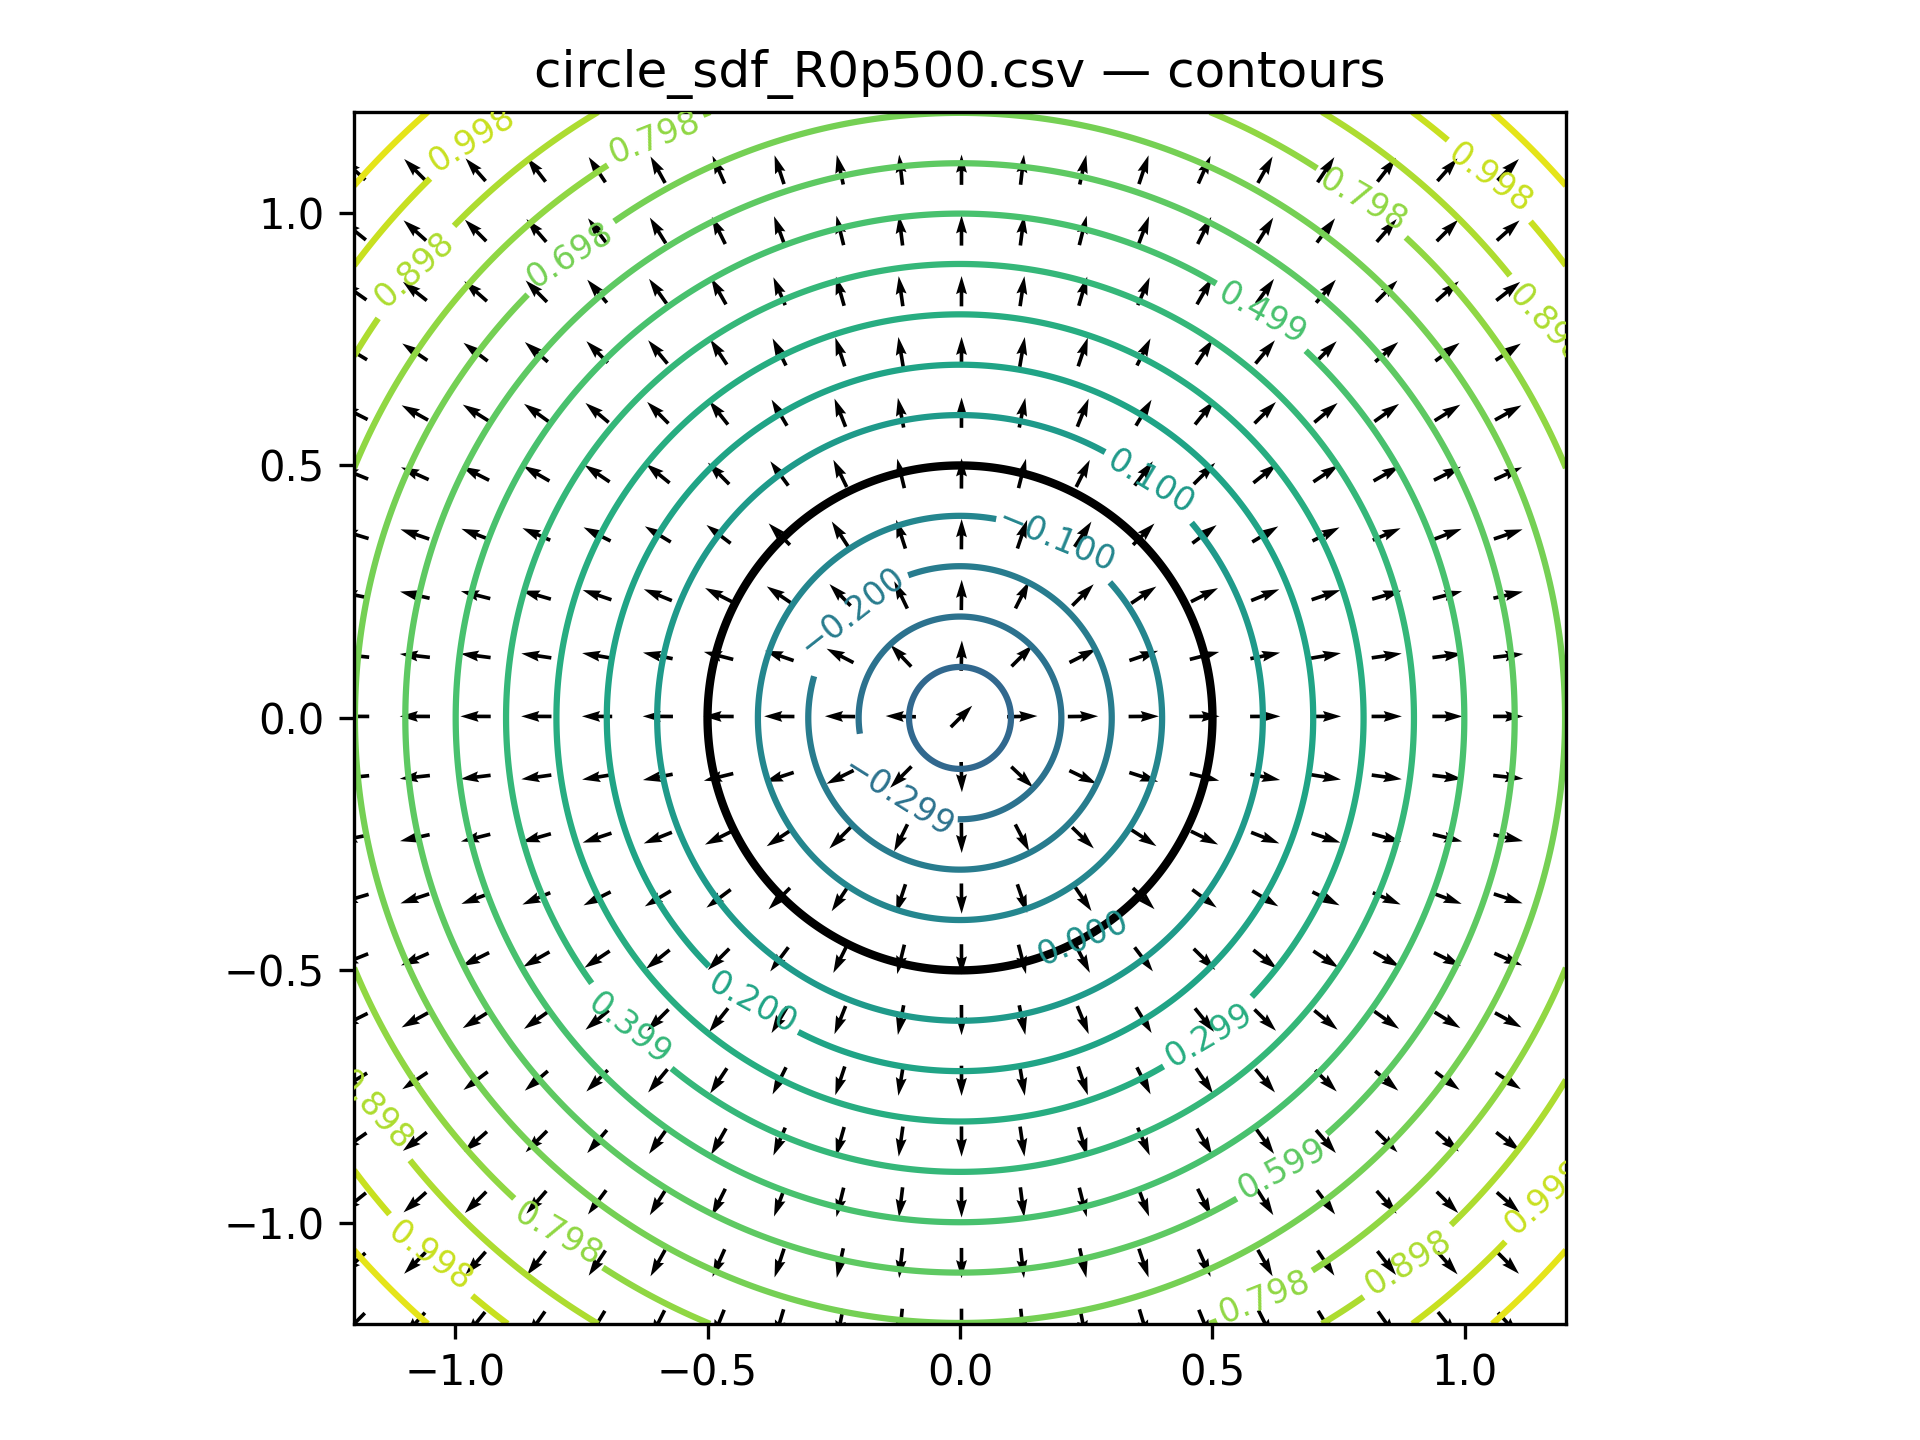
\includegraphics[width=\linewidth]{Figures/circle_sdf_R0p500_contour.png}\\[-0.2em]
          \scriptsize Circle — contour
        \end{minipage}
      \end{minipage}
    \end{column}
  \end{columns}
\end{frame}

% --- Method Overview ---
\begin{frame}{Method Overview}
\begin{columns}[T,onlytextwidth]
    % ================= LEFT: OBJECT =================
    \begin{column}{0.5\textwidth}
        \textbf{Object-side optimization}
        \[\begin{aligned}
        \min_{\{c_{t:T}\},\,\{\lambda_{t:T}\},\,\{T_{t:T}\}} \;\; 
        & J_{O}(T_{0}, T^*, c, \lambda)
        \end{aligned}\]
        \[
        \text{s.t.}\quad
        \begin{aligned}
        & f(c,\lambda) = 0 \\
        & g_i(c,\lambda) \ge 0,\; i\in\mathcal{I} \\
        & g_i(c,\lambda) = 0,\; i\in\mathcal{E} \\
        & 0 \le \phi(c) \;\perp\; \lambda \ge 0 \quad
        \end{aligned}
        \]
        \textbf{Where (object):}
        \begin{itemize}\itemsep0.1em
            \item $J_{O}$ object cost function
            \item $T_0$ (initial object pose), $T^*$ (goal object pose)
            \item $c_t$ (contact point), $\lambda_t$ (contact force)
            \item $f(\cdot)$ (object's dynamics), $g(\cdot)$ (constraints)
            \item $\phi(\cdot)$ (object's signed distance function)
        \end{itemize}
    \end{column}
    
    % ================= RIGHT: ROBOT =================
    \begin{column}{0.5\textwidth}
        \textbf{Robot-side optimization}
        \[\begin{aligned}
        \min_{\{u_{t:T}\}} \;\; 
        & J_{R}(T_0, T^*, c, \lambda, \phi(\cdot), q_{0}, u_{0})
        \end{aligned}\]
        \[ \text{s.t.}\quad
        \begin{aligned}
        & u_{\min}\!\le u_t \le u_{\max} \\
        & q_{\min}\!\le q_t \le q_{\max} \\
        & \|v_t\|\le v_{\max} \\
        \\
        \end{aligned}\]
        
        \medskip
        \textbf{Where (robot):}
        \begin{itemize}\itemsep0.1em
            \item $J_{R}$ robot cost function
            \item $T_0$ (initial object pose), $T^*$ (goal object pose)
            \item $c_t$ (contact point), $\lambda_t$ (contact force)
            \item $\phi(\cdot)$  (object's signed distance function)
            \item $q_0$ (initial joints), $u_0$ (initial joint controls)
        \end{itemize}
    \end{column}
\end{columns}
\end{frame}

\begin{frame}[plain]
  \centering
  \Huge Robot-level Optimization
\end{frame}

% --- MPC Formulation ---
\begin{frame}{MPC Formulation}
\begin{enumerate}[<+->]
    \item \textbf{Problem Setup} 
        \begin{itemize}[<.->]
            \item State dynamics: $x_{t+1} = f(x_t, u_t)$, \quad $t=0,\dots,T-1$ 
            \item Objective: $\min \; J = \sum_{t=0}^{T-1} \ell_t(x_t,u_t) + \ell_T(x_T)$  
        \end{itemize}

    \item \textbf{Stage Costs}  
    \begin{itemize}[<.->]
      \item Goal tracking: $\ell_{\text{goal}} = \|T_{\text{goal}} - T_{\text{obj},k}\|_2^2$
      \item Stabilizers: effort $\ell_{\text{eff}}$, smoothness $\ell_{\text{smooth}}$
      \item Speed caps near contact: $\ell_{\text{spd}}$
      \item End-Effector Pose: $\ell_{\text{rpy}}$
    \end{itemize}

    \item \textbf{Closed-Loop Receding Horizon} 
        \begin{enumerate}[<.->]
            \item Sample $K$ control sequences $\{u_{t:t+T-1}^{(k)}\}$
            \item Roll out dynamics
            \item Score with cost terms
            \item Update parameters $\&$ controls $\{u_{t:t+T-1}^{(k)}\}$
        \end{enumerate}
        
    \item \textbf{Safety \& Constraints}  
    \begin{itemize}[<.->]
      \item Hard bounds on $u_t$ and $q_t$ 
    \end{itemize}
\end{enumerate}
\end{frame}

% --- Sampling-Based Motion Planning ---
\section{Sample-Based Motion Planning}
% MPPI
\subsection{MPPI}
\begin{frame}{Model Predictive Path Integral (MPPI)\,\footnotemark[1]}
  \begin{enumerate}
    \item \textbf{Idea:}  
    Treat control optimization as a weighted average over noisy rollouts

    \item \textbf{Algorithm:}  
    \begin{itemize}
      \item Sample $K$ control sequences: $\{u_{t:t+T-1}^{(k)}\}$
      \item Roll out dynamics: $x_{t+1}=f(x_t,u_t)$
      \item Evaluate trajectory cost $J^{(k)} = \sum \ell(x_t,u_t)$
      \item Weight by exponential transform:  
      $w^{(k)} = \exp\!\Big(-\tfrac{1}{\lambda} J^{(k)}\Big)$
      \item Update control:  
      $u_t \leftarrow \frac{\sum_k w^{(k)} u_t^{(k)}}{\sum_k w^{(k)}}$
    \end{itemize}

    \item \textbf{Properties:}  
    \begin{itemize}
      \item No need for gradients $\Rightarrow$ robust to nonsmooth costs
      \item Naturally parallelizable (GPU rollouts)
      \item Handles nonconvex landscapes
    \end{itemize}
  \end{enumerate}

  \footnotetext[1]{\scriptsize Williams, G., Aldrich, A., \& Theodorou, E. A. (2015).
  \emph{Model Predictive Path Integral Control using Covariance Variable Importance Sampling}.
  \href{https://arxiv.org/abs/1509.01149}{arXiv:1509.01149}.}
\end{frame}

\begin{frame}{Model Predictive Path Integral (MPPI)}
\end{frame}

% % CEM
% \subsection{CEM}
% \begin{frame}{Cross-Entropy Method (CEM)}
%       \begin{enumerate}
%         \item \textbf{Idea:}  
%         Iteratively improve a sampling distribution by focusing on the best-performing “elite” rollouts.

%         \item \textbf{Algorithm:}  
%         \begin{itemize}
%           \item Sample $K$ control sequences from Gaussian $\mathcal{N}(\mu,\Sigma)$
%           \item Roll out dynamics, compute costs $J^{(k)}$
%           \item Select top-$M$ elite samples with the lowest cost
%           \item Refit Gaussian to elites:  
%           $\mu \leftarrow \frac{1}{M}\sum_{k \in \text{elite}} u^{(k)}$,  
%           $\Sigma \leftarrow \text{Cov}\big(u^{(k)}\big)$
%           \item Repeat until convergence (or horizon shift)
%         \end{itemize}

%         \item \textbf{Properties:}  
%         \begin{itemize}
%           \item Deterministic update from elites
%           \item Efficient when the elite set is informative
%           \item Requires fewer hyperparameters than MPPI
%         \end{itemize}
%       \end{enumerate}
% \end{frame}

% Reward Design
\begin{frame}{Reward Design}
    \small
    \begin{enumerate}
      \item \textbf{Goal Shaping} $J_{\text{goal}} = \|T_{\text{goal}} - T_{\text{obj}}\|_2$
      \item \textbf{Smoothness \& Effort} $J_{\text{eff}} = \|u_t\|_2^2,\quad J_{\text{smooth}} = \|\Delta u_t\|_2^2$
    
      \item \textbf{Distance-Adaptive Speed Cap}  
      \[
      \begin{aligned}
      &d_t = \max\{0,\ \phi(p^{\mathrm{ee}}_t;\,T_{\text{obj}})\} \quad \text{(object SDF)} \\
      &v_{\text{cap}}(d_t) = v_{\text{near}} + (v_{\text{far}}-v_{\text{near}})\,
        \sigma\!\left(\frac{d_t - d_{\text{near}}}{\tau}\right),\quad
        \sigma(z)=\tfrac{1}{2}(1+\tanh z) \\
      &\boxed{\,J_{\text{spd}} = \big[\max(0,\ \|v^{\mathrm{ee}}_t\| - v_{\text{cap}}(d_t))\big]^2\,}
      \end{aligned}
      \]
    
      \item \textbf{End-Effector Uprightness (roll/pitch)} $\,J_{\text{rpy}} = \phi_t^2 + \theta_t^2 $ \
    \end{enumerate}
    
    \medskip
    \textbf{Total:}\,
    $J = w_{\text{goal}} J_{\text{goal}}
     + w_{\text{eff}} J_{\text{eff}}
     + w_{\text{smooth}} J_{\text{smooth}}
     + w_{\text{speed}} J_{\text{speed}}
     + w_{\text{rpy}} J_{\text{rpy}}$
    
    \medskip
    \textbf{Where:}
    $v_{\text{far}}>v_{\text{near}}>0$; $d_{\text{near}}$ is where slowing begins; $\tau$ controls transition sharpness
\end{frame}

\begin{frame}[plain]
  \centering
  \Huge Object-level Optimization
\end{frame}

% --- CRISP ---
\section{CRISP}
\subsection{CRISP Formulation}
% Object Modeling
\begin{frame}{Object Modeling}
    \begin{enumerate}
        \item \textbf{Dynamic Model (Equality Constraints)}  
        \[
          x_{t+1} = f(x_t, u_t), \quad 
          x = [p_x, p_y, \theta], \quad 
          u = [c_x, c_y, \lambda]
        \]  
      \vspace{1.5em}
        
        \item \textbf{Contact Constraints (Inequalities)}  
        \[
          \phi(x) \geq 0, \quad 
          \lambda \geq 0, \quad 
          -\phi(x)\,\lambda \geq 0
        \]  
      \vspace{1.5em}
        
        \item \textbf{Initial Constraints}  
        \[ x(0) = x_0 \]  
    \end{enumerate}

\end{frame}

% Object Kinematics and Dynamics (Equality Constraints)
\begin{frame}{Object Kinematics and Dynamics (Equality Constraints)}
      \small 
      \textbf{State \& control (per step $t$):}
      \[
        x_t = \begin{bmatrix} p_{x,t} \\ p_{y,t} \\ \theta_t \end{bmatrix},
        \qquad
        u_t = \begin{bmatrix} c_{x,t} \\ c_{y,t} \\ \lambda_{1-4,t} \end{bmatrix}  \text{(analytical)}
      \]
      with objects center $p$, object orientation $\theta$, contact location $c$ and applied force $\lambda$ \medskip

      \textbf{Discrete-time dynamics (explicit Euler):}
      \[\begin{aligned}
          \mathbf{p}_{t+1} &= \mathbf{p}_t + \Delta t\,\dot{\mathbf{p}}_t,
          &\qquad
          \theta_{t+1} &= \theta_t + \Delta t\,\dot\theta_t,
        \end{aligned}\]
      where $\mathbf{p}_t=[p_{x,t},p_{y,t}]^\top$ and time step $\Delta t$\medskip

      \textbf{Forces/torque from contact:}
        \[
            \dot{\mathbf{p}}_t = \frac{1}{\mu m g}\,\mathbf{F}^{\text{world}}_t,
            \qquad
            \dot\theta_t = \frac{\tau_t}{J_z}
        \]
        where $J_z$ is angular scalar $1/(\mu m g)$ ($m$-mass, $\mu$-friction, and $g$-gravity) 

     \textbf{Equality constraints (per $t=0{:}T-1$):}
      \[
        g^{\text{dyn}}_t(x_t,u_t) \;=\;
        \begin{bmatrix}
          \mathbf{p}_{t+1} - \mathbf{p}_t - \Delta t\,\dot{\mathbf{p}}_t\\[0.2em]
          \theta_{t+1} - \theta_t - \Delta t\,\dot\theta_t
        \end{bmatrix} = \mathbf{0}.
      \]
\end{frame}

% Object Dynamics Model Analytical
\begin{frame}{Object Dynamics Model (Analytical)}
  \begin{columns}[T,onlytextwidth]
    \begin{column}{0.72\textwidth}
      \emph{Analytical “face” model uses face-aligned direction}
      \[
        \underbrace{\mathbf{F}^{\text{body}}_t}_{\in\mathbb{R}^2}
        =
        \begin{bmatrix}
          \lambda_{2,t}+\lambda_{4,t}\\[0.2em]
          \lambda_{1,t}+\lambda_{3,t}
        \end{bmatrix},
        \qquad
        \mathbf{F}^{\text{world}}_t = R(\theta_t)\,\mathbf{F}^{\text{body}}_t
      \]
      \[
        \tau_t
        = \underbrace{c_{x,t}}_{r_x}\,\,\underbrace{(\mathbf{F}^{\text{body}}_t)_y}_{\lambda_{1,t}+\lambda_{3,t}}
          \;-\;
          \underbrace{c_{y,t}}_{r_y}\,\,\underbrace{(\mathbf{F}^{\text{body}}_t)_x}_{\lambda_{2,t}+\lambda_{4,t}}
      \]

      \textbf{Where:}  \\
      $R(\theta)=\begin{bmatrix}\cos\theta & -\sin\theta\\ \sin\theta & \cos\theta\end{bmatrix}$  \\
      
    \end{column}

    \begin{column}{0.28\textwidth}
      \centering
      {\bfseries Problem Setup}\footnotemark\\[0.5em]
      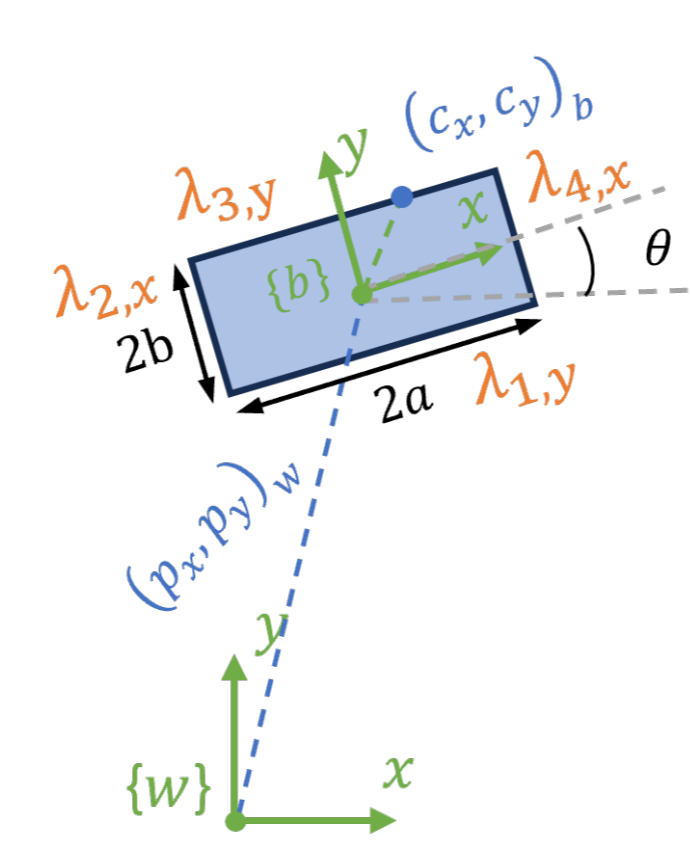
\includegraphics[width=\textwidth]{Figures/pushbox_crisp_example_analytical.png}
    \end{column}
  \end{columns}

  \footnotetext{\scriptsize Image adapted from Li et al. (2025), \emph{CRISP}, \href{https://arxiv.org/abs/2502.01055}{arXiv:2502.01055}.}
\end{frame}

% Object Dynamics Model SDF
\begin{frame}{Object Dynamics Model (SDF)}
  \begin{columns}[T,onlytextwidth]
    \begin{column}{0.65\textwidth}
      \small
      \emph{SDF-normal model for arbitrary shapes}
      \begin{align*}
        \textbf{(controls)}\quad
        u_t &= \begin{bmatrix} c_{x,t} \\ c_{y,t} \\ \lambda_t \end{bmatrix} \\ 
        \textbf{(normal)}\quad
        \mathbf{n}^b_t &= -\frac{\nabla\phi(\mathbf{c}_t)}{\|\nabla\phi(\mathbf{c}_t)\|} \\[0.15em]
        \textbf{(linear force)}\quad
        \mathbf{F}^b_t &= \lambda_t\,\mathbf{n}^b_t, \quad \mathbf{F}^w_t = R(\theta_t)\,\mathbf{F}^b_t \\[0.15em]
        \textbf{(torque about COM)}\quad
        \tau_t &= \big(c_{x,t} n^b_{y,t} - c_{y,t} n^b_{x,t}\big)\,\lambda_t \\[0.15em]
      \end{align*}

      \textbf{Where:} the sign on $\mathbf{n}^b_k$ is flipped so that SDF gradient points inward.
    \end{column}

    \begin{column}{0.35\textwidth}
      \centering
      {\bfseries Problem Setup}\\[0.4em]
      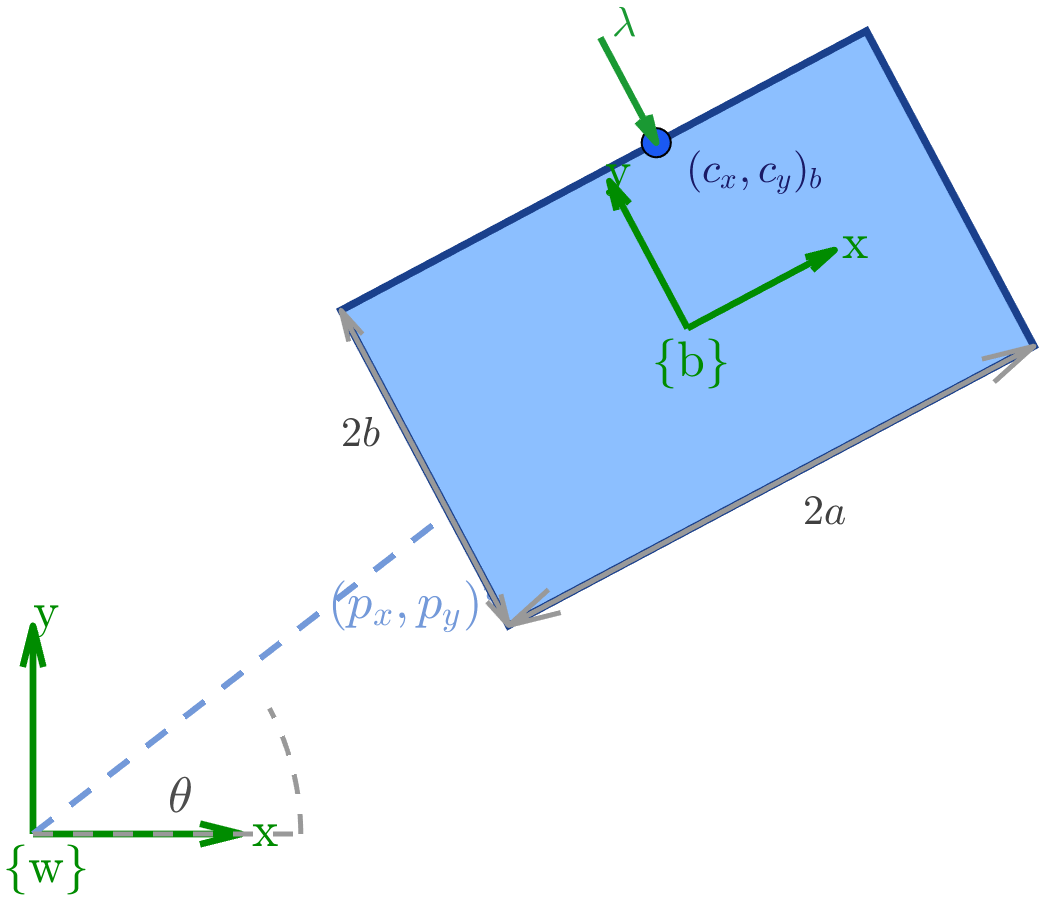
\includegraphics[width=\linewidth]{Figures/pushbox_crisp_example_sdf.png}

      \vspace{0.4em}
      \footnotesize
      \begin{tabular}{@{}l@{}}
        $\{w\}$ world frame \quad $\{b\}$ body frame
      \end{tabular}
    \end{column}
  \end{columns}
\end{frame}

% Object Shape and Contact 
\begin{frame}{Object Shape and Contact}
      \textbf{SDF sign convention} \\
      $\phi(\mathbf{p}) > 0$ outside the object \\
      $\phi(\mathbf{p}) = 0$ on the surface \\
      $\phi(\mathbf{p}) < 0$ inside
      \vspace{1.5em}
      
      \textbf{Contact constraints (per step $t$)}
      \[
        \phi(\mathbf{c}_t) \ge 0,\quad
        \lambda_t \ge 0,\quad
        \lambda_t\,\phi(\mathbf{c}_t) \approx 0
      \]
      {\footnotesize (non-penetration, nonnegative normal force, force only at contact; “$\approx 0$”)}
      \vspace{1.5em}
      
      \textbf{Initial constraints}
      \[ x(0) = {x}_0 \]
      {\footnotesize (enforce start pose and any prescribed initial contacts)}
\end{frame}

% Object-Level Optimization via CRISP
\begin{frame}{Object-Level Optimization via CRISP\,\footnotemark[1]}
  \begin{columns}[T,onlytextwidth]
    % ---------------- LEFT: problem ----------------
    \begin{column}{0.46\textwidth}
      \small
      \textbf{Problem Formulation \quad \footnotesize\color{gray}{(Eq.~6)}}
      \[
      \begin{aligned}
        &\min_{c,\lambda}\; J(c,\lambda) \\
        \text{s.t.}\;& f(c,\lambda) = 0 \quad &&\text{(dynamics/defects)} \\
                     & g_i(c,\lambda) \ge 0,\; i\in\mathcal{I} \quad &&\text{(ineq.)} \\
                     & g_i(c,\lambda) = 0,\; i\in\mathcal{E} \quad &&\text{(eq.)} \\
                     & 0 \le \phi(c,\lambda) \;\perp\; \lambda \ge 0 \quad &&\text{(complementarity)}
      \end{aligned}
      \]
      \footnotesize
      \textbf{Where:} \\
      \begin{itemize}
          \item $x\!=\!(v,\lambda)$ trajectory and contact forces
          \item $\phi(\cdot)$ is the gap function (SDF) 
          \item $\lambda\!\ge\!0$ are normal forces
          \item $f,g_i$ dynamics and other constraints 
      \end{itemize}
    \end{column}

    % ---------------- RIGHT: merit + steps ----------------
    \begin{column}{0.54\textwidth}
      \small
      \textbf{Merit function (weighted $\mu$) \quad \footnotesize\color{gray}{(Eq.~8)}}
      \[
        \varphi_1(x;\mu) \;=\; J(x)
        + \sum_{i\in\mathcal{E}} \mu_i\,|g_i(x)|
        + \sum_{i\in\mathcal{I}} \mu_i\,[g_i(x)]^{-},
      \]
      \vspace{-1.0em}
      \[ [g]^{-} = \max\{0,-g\},\qquad \mu_i>0  \]
      \vspace{-0.4em}

      \textbf{Algorithm sketch (per iteration $t$)}
      \begin{enumerate}\setlength{\itemsep}{0.15em}
        \item Linearize $f,g$ at $x^{(t)}$; build trust-region SQP
        \item Handle complementarity via penalties in $\varphi_1$
        \item Solve for step $p^{(t)}$; compute predicted vs. actual decrease of $\varphi_1$
        \item Accept/Reject step; shrink/expand trust region
        \item Update penalties $\mu \uparrow$ for violated constraints 
        \item Check convergence: merit decrease + constraint violation/KKT residual
      \end{enumerate}
    \end{column}
  \end{columns}

\footnotetext[1]{\scriptsize Li, Y., et al. (2025).
\emph{\href{https://arxiv.org/abs/2502.01055}{On the Surprising Robustness of Sequential Convex Optimization for Contact-Implicit MP}}}
  
\end{frame}

% CRISP: Optimization (SQP I)
\begin{frame}{CRISP: Optimization — SQP with Merit (I)}
  \small
  \textbf{Build the subproblem (linearize constraints at $x^{(k)}$):}
  \[
    \min_{p_k}\ \tfrac12 p_k^\top H^{(k)} p_k + \nabla J(x^{(k)})^\top p_k
    \quad\text{s.t.}\quad
    \begin{aligned}
      &f(x^{(k)})+\nabla f(x^{(k)})\,p_k=0,\\
      &g(x^{(k)})+\nabla g(x^{(k)})\,p_k\ge 0,\\
      &\|p_k\|\le \Delta^{(k)}.
    \end{aligned}
  \]

  \textbf{CRISP quadratic model of the merit:}
  \[
    \min_{p_k}\; \underbrace{J_k+\nabla J_k^\top p_k+\tfrac12 p_k^\top \nabla^2_{xx}J_k\,p_k}_{\text{quadratic model of }J}
    +\!\!\sum_{i\in\mathcal E}\!\mu_i\big|g_i(x_k)+\nabla g_i(x_k)^\top p_k\big|
    +\!\!\sum_{i\in\mathcal I}\!\mu_i\,[g_i(x_k)+\nabla g_i(x_k)^\top p_k]^{-}
  \]
  \[
    \text{s.t.}\quad f(x_k)+\nabla f(x_k)\,p_k=0,\qquad \|p_k\|\le \Delta^{(k)}.
  \]

  \vspace{0.2em}
  {\footnotesize $J_k,\nabla J_k,\nabla^2_{xx}J_k$ evaluated at $x_k$.}
\end{frame}

% CRISP: Optimization (SQP II)
\begin{frame}{CRISP: Optimization — Local Merit Model (II)}
  \small
  \textbf{Step acceptance via merit ratio:}
  \[
    \text{pred}=\varphi_1(x^{(k)};\mu)-m^{(k)}(p_k), \quad
    \text{ared}=\varphi_1(x^{(k)};\mu)-\varphi_1(x^{(k)}\!+\!p_k;\mu), \quad
    \rho=\frac{\text{ared}}{\text{pred}}
  \]

  \textbf{Trust-region ($\gamma$) acceptance \& radius update:}
  \[
    x^{(k+1)}=
    \begin{cases}
      x^{(k)}+p_k, & \rho\ge \eta\\
      x^{(k)}, & \rho<\eta
    \end{cases}
    \qquad
    \Delta^{(k+1)}=
    \begin{cases}
      \gamma_{\uparrow}\Delta^{(k)}, & \rho\text{ large}\\
      \gamma_{\downarrow}\Delta^{(k)}, & \rho\text{ small}\\
      \Delta^{(k)}, & \text{otherwise}
    \end{cases}
  \]
  
  \textbf{Penalty update \& convergence:}
  \begin{itemize}\setlength{\itemsep}{0.2em}
    \item Increase $\mu_i$ for constraints whose violations stagnate (cap at $\mu_{\max}$)
    \item Stop when merit decrease and KKT/violations are small (exact-penalty $\rightarrow$ near a KKT point)
  \end{itemize}
  
  {\footnotesize Complementarity handled via relaxation/penalty inside $\varphi_1$ or an nonlinear complementarity problem (NCP)}
\end{frame}

% --- Reward Design from SDF + CRISP  ---
\subsection{Reward Design from SDF + CRISP}
\begin{frame}{Reward Design from SDF + CRISP}

  \begin{enumerate}[<+->]
    \item \textbf{SDF for Geometric Safety}  
    \begin{itemize}[<.->]      
        \item \textbf{Collision \& Clearance}  
        $J_{\text{obs}} = \sum \max(0,\, d_{\text{safe}} - \phi(c_t))$
        \item \textbf{Contact Directionality}  
        Encourage pushes aligned with surface normal $\nabla \phi$
        \item \textbf{Penetration Handling} Large penalty for $\phi(c_t) < 0$ (inside obstacle)
    \end{itemize}

    \item \textbf{Trajectory-based Reward from CRISP}\\
    Compare predicted contact-point trajectories with object trajectory from MPPI rollout $\Rightarrow$ reward signal for control sequence

    \item \textbf{Hybrid Reward}  
    \[ J = \alpha J_{\text{CRISP}} + (1-\alpha) J_{\text{SDF}} \]

    \item \textbf{Benefits}  
    \begin{itemize}[<.->]
      \item CRISP: task-aware, interpretable phases
      \item SDF: geometry-aware, safe by design
      \item Combined: structured and robust
    \end{itemize}
  \end{enumerate}
\end{frame}

\begin{frame}{Task: Push Rectangle}
\end{frame}
\begin{frame}{Task: Push Box}
\end{frame}
\begin{frame}{Task: Push Box}
\end{frame}
\begin{frame}{Task: Push Box}
\end{frame}
\begin{frame}{Task: Push Box SDF}
\end{frame}
\begin{frame}{Task: Pull Circle SDF}
\end{frame}
\begin{frame}{Task: Push Circle SDF}
\end{frame}

% --- Approach ---
\section{Approach}
\begin{frame}{Approach: Chart}
\end{frame}

% --- Task Suite ---
% Task A
\section{Task Suite}
\subsection{Task A: Push Cube with Cube}
\begin{frame}{Task A: Push Cube with Cube}
  \begin{columns}[T]
    \begin{column}{0.6\textwidth}
      \begin{block}{Objective}
        Translate the object of interest to the goal with minimal collisions and in a short time
      \end{block}
    \end{column}

    \begin{column}{0.4\textwidth}
    \end{column}
  \end{columns}
\end{frame}
\begin{frame}{Task: MPPI}
\end{frame}
\begin{frame}{Task: MPPI + CRISP without tip}
\end{frame}
\begin{frame}{Task: MPPI + CRISP with tip}
\end{frame}
\begin{frame}{Task: MPPI + CRISP with tip}
\end{frame}
\begin{frame}{Task: MPPI + CRISP challange MPPI}
\end{frame}
\begin{frame}{Task: MPPI + CRISP challange MPPI}
\end{frame}
\begin{frame}{Task: MPPI + CRISP challange CRISP}
\end{frame}
\begin{frame}{Task: MPPI + CRISP SDF}
\end{frame}

% Task B
\subsection{Task B: Push Cube with Xarm6}
\begin{frame}{Task B: Push Cube with Xarm6}
  \begin{columns}[T]
    \begin{column}{0.6\textwidth}
      \begin{block}{Objective}
        Perform \textbf{end-effector mediated pushing} of the cube while respecting manipulator kinematic limits
      \end{block}

      \vspace{1em}

      \begin{block}{Key Challenges}
        \begin{itemize}
          \item \textbf{Link clearance} — avoid collisions along arm geometry  
          \item \textbf{Contact placement} — selecting stable push points
          \item \textbf{Wrist alignment} — aligning end-effector normal with surface
        \end{itemize}
      \end{block}
    \end{column}

    \begin{column}{0.4\textwidth}
    \end{column}
  \end{columns}
\end{frame}

\begin{frame}{Task: MPPI}
\end{frame}
\begin{frame}{Task: CRISP + IK}
\end{frame}

% --- Evaluation Protocol ---
\section{Evaluation Protocol}
\begin{frame}{Evaluation Protocol}
  \begin{block}{Metrics}
    \begin{itemize}
      \item \textbf{Success rate} — fraction of trials reaching goal within some translation and orientation margin
      \item \textbf{Time-to-goal} — execution time until task completion
      \item \textbf{Path length} — distance traveled by object/EE
      \item \textbf{Peak penetration} — maximum signed distance violation
      \item \textbf{Constraint violations} - equality and inequality constraint violation
      \item \textbf{Contact smoothness} — stability of forces/trajectories
    \end{itemize}
  \end{block}

  \begin{block}{Comparisons}
    \begin{itemize}
      \item Baselines: (i) CRISP + IK, (ii) MPPI SDF-only, (iii) CRISP+MPPI
      \item Ablations: horizon $T$, samples $K$, temperature $\lambda$,  
            clearance margin, normal-alignment
    \end{itemize}
  \end{block}

  \begin{block}{Runtime Reporting}
    \begin{itemize}
      \item Average latency per step
      \item Wall-clock task completion time
    \end{itemize}
  \end{block}
\end{frame}

% --- Results ---
\section{Results}
\begin{frame}{Results}
  \begin{block}{Quantitative Results}
    \begin{itemize}
      \item \textbf{Success vs. samples $K$}: MPPI $\Rightarrow$ higher $K$ improves success
      \item \textbf{Baseline comparison}: (i) CRISP + IK, (ii) MPPI SDF-only, (iii) CRISP+MPPI $\Rightarrow$ CRISP improves robustness by guiding the contact, resulting in fewer failure modes
      \item \textbf{Runtime scaling}: parallel rollouts (CPU/GPU) $\Rightarrow$ near real-time performance
    \end{itemize}
  \end{block}

  \vspace{0.5em}

  \begin{block}{Qualitative Results}
    \begin{itemize}
      \item Trajectories of contact points and object motion
      \item Surface normals aligned at contact
      \item SDF slices show safe clearance and penetration handling
    \end{itemize}
  \end{block}
\end{frame}

% --- Limitations and Failure Modes ---
\section{Limitations \& Failure Modes}
\begin{frame}{Limitations \& Failure Modes}
  \begin{block}{Observed Issues}
    \begin{itemize}
      \item \textbf{Suboptimal CRISP trajectory:}  \\
            CRISP could provide a suboptimal path of the contact trajectory that leads to a longer way, even when obstacles are not present
      \item \textbf{MPPI:} \\ 
            MPPI samples do not have to be optimal and are highly dependent on the samples and the horizon
      \item \textbf{CRISP + MPPI:} \\
            Leads to a decent trajectory, but the reward sometimes causes the MPPI to focus too much on following CRISP rather than improving the initial goal objective
    \end{itemize}
  \end{block}

  \vspace{0.5em}

  \begin{block}{Takeaway}
    Robustness improves with CRISP+MPPI, but failure modes remain in cases where the contact has to produce a large force to move the object
  \end{block}
\end{frame}

% --- Conclusion ---
\section{Conclusion}
\begin{frame}{Conclusion}
  \begin{block}{Key Insights}
    \begin{itemize}
      \item \textbf{Contact-implicit planning is hard:}  
            non-convex geometry, mode switches, friction cones
      \item \textbf{Signed Distance Functions (SDF):}  
            provide distances and normals $\nabla \phi$ for smooth, geometry-aware rewards
      \item \textbf{Sample-based control (MPPI):}  
            robust in non-convex landscapes, avoids mode enumeration
      \item \textbf{CRISP + MPPI:}  
            combines structured task guidance with geometric safety
            $\Rightarrow$ higher success rates
    \end{itemize}
  \end{block}

  \vspace{0.5em}

  \begin{block}{Takeaway}
    CRISP provides a \textbf{guided contact trajectory}, which MPPI follows using SDF-based rewards (goal distance, clearance, alignment). Together, they yield contact-rich behaviors that are \emph{structured, safer, and more effective}
  \end{block}
\end{frame}

% --- Future Work ---
\section{Future Work}
\begin{frame}{Future Work}
\begin{columns}
    \begin{column}{0.8\textwidth}   
        \begin{block}{Near-Term Extensions}
        \begin{itemize}
          \item Perform simulations on \textbf{XArm6} with SDF-based MPC
          \item Extend to \textbf{multi-object tasks}, bimanual setups, and mobile manipulators
        \end{itemize}
        \end{block}
        
        \vspace{0.5em}
        
        \begin{block}{Modeling Improvements}
        \begin{itemize}
          \item Upgrade CRISP with SDF and inertia-aware dynamics for general shapes
          \item Explore learned/neural SDFs for richer geometry
          \item Incorporate tactile sensing for normal estimation
        \end{itemize}
        \end{block}
        
        \vspace{0.5em}
        
        \begin{block}{Towards Real Systems}
        \begin{itemize}
          \item \textbf{Sim-to-real transfer:} domain randomization, online SDF updates
          \item Extend to grasping and re-grasping with contact switching
        \end{itemize}
        \end{block}
    \end{column}

    \begin{column}{0.3\textwidth}
      \centering
      {\bfseries Reachy 2}\\[0.4em]
      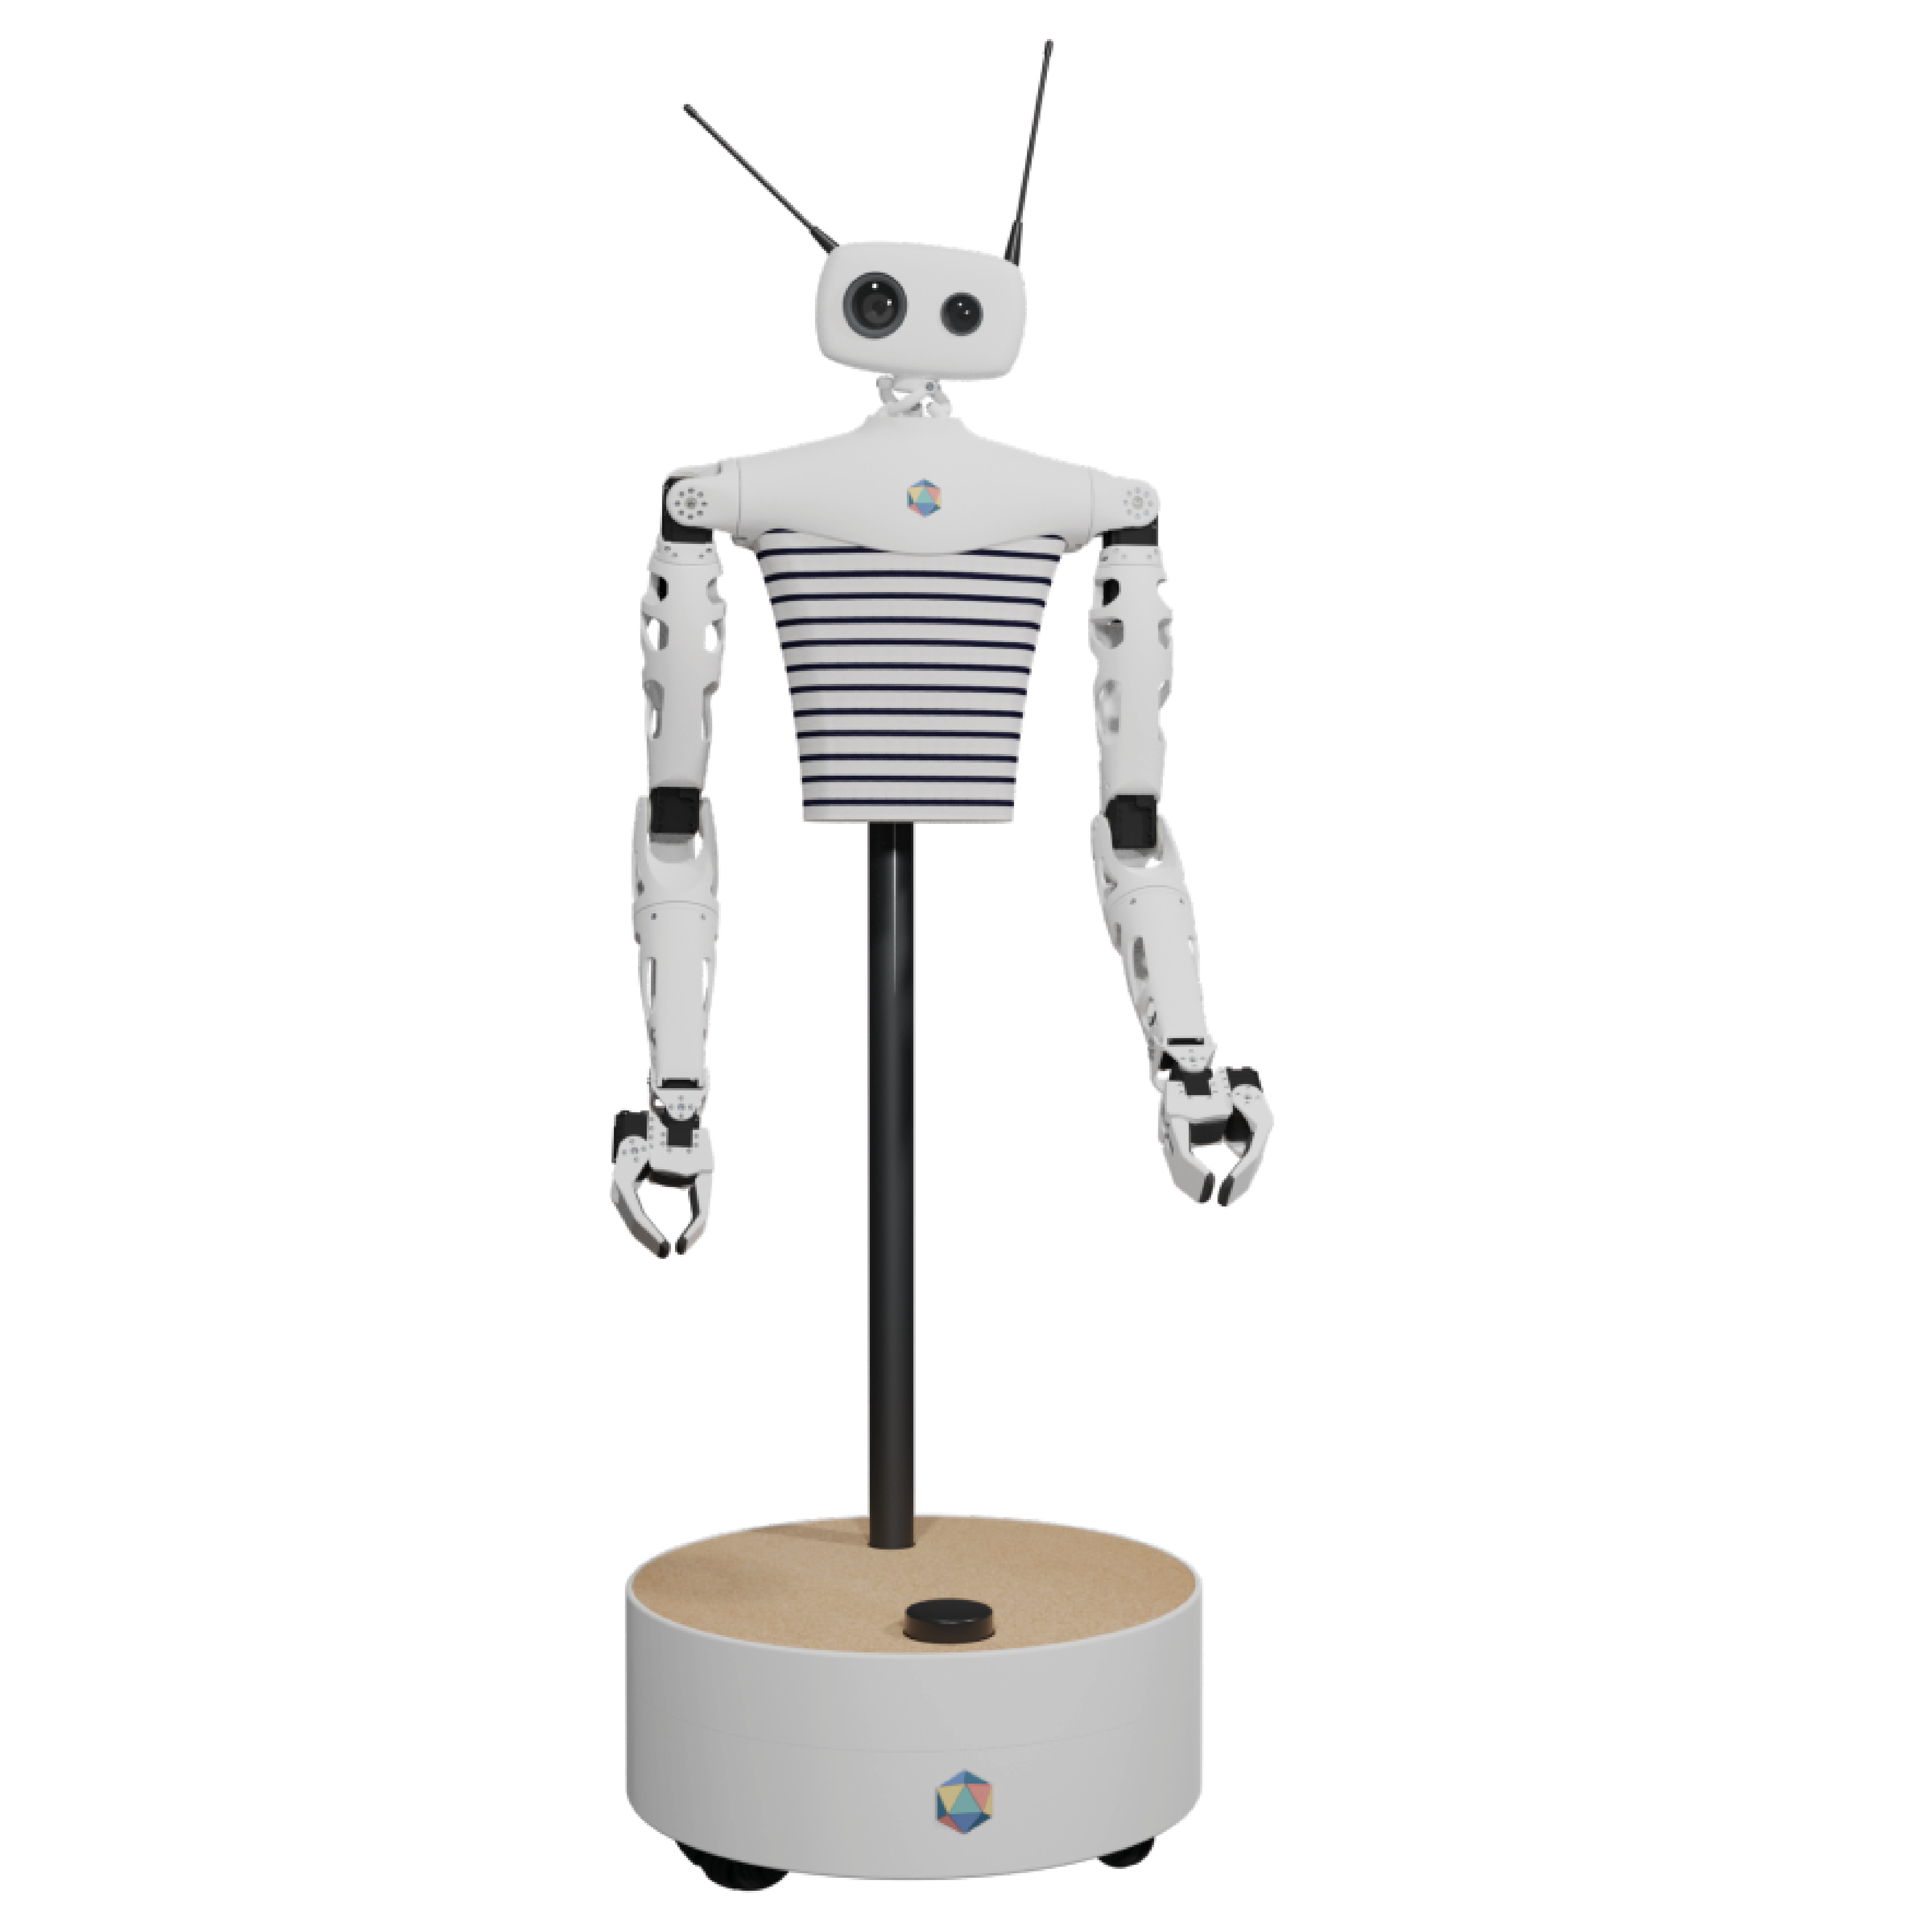
\includegraphics[width=\linewidth]{Figures/reachy_02.png}
    \end{column}
\end{columns}
\end{frame}

% --- Thank You Slide ---
\begin{frame}[plain] 
  \centering
  \vfill
  {\Huge \textbf{Thank You!}} \\[1.5em]
  {\Large Questions?} \\[3em]

  {\small
    \texttt{nmarinosraitsevits@ucsd.edu} \\
  }
  \vfill
\end{frame}

\end{document}



